\documentclass[conference]{IEEEtran}

\IEEEoverridecommandlockouts

\usepackage{cite}
\usepackage{amsmath,amssymb}
\usepackage{graphicx}
\usepackage{booktabs}
\usepackage{url}
\usepackage{float}

\begin{document}

\title{Classroom Reaction Recognition Using Transfer Learning with ResNet18 and VGG16}

\author{%
\IEEEauthorblockN{Umman Mammadov\textsuperscript{1},
Anar Bastanov\textsuperscript{1}, and
Anar Shirinov\textsuperscript{1}}
\IEEEauthorblockA{\textsuperscript{1}\textit{AI and ML Fundamentals},
Baku Higher Oil School (BHOS)\\
\texttt{\{umman.mammadov, anar.bastanov, anar.shirinov\}.std@bhos.edu.az}}}

\maketitle

% -----------------------------------------------------------------
\begin{abstract}
We built an end-to-end pipeline that takes raw classroom video, detects students with YOLOv8-nano, and classifies each person's facial reaction into five classes: Neutral, Confused, Smiling/Amused, Surprised, and Bored/Tired. We fine-tuned two pretrained models---ResNet18 and VGG16---and compared them under identical conditions. ResNet18 reached 90.0\% test accuracy (F1 0.900), outperforming VGG16 at 87.3\% (F1 0.874). The best model was exported to ONNX for fast CPU inference ($2.89\times$ speedup) and a reference AWS architecture was designed for scalable deployment.
\end{abstract}

\begin{IEEEkeywords}
facial expression recognition, transfer learning, ResNet, VGG, YOLOv8, ONNX, classroom analytics
\end{IEEEkeywords}

% -----------------------------------------------------------------
\section{Introduction}

Understanding how students react during lectures helps instructors get real-time feedback and adjust their teaching. Traditional methods like manual observation or surveys do not scale and miss the moment-to-moment dynamics of student attention.

This project uses computer vision to automate that process. We recorded a real university lecture, detected individual students in each frame, manually labeled their facial reactions, and trained two deep learning models to classify them. The entire pipeline---from raw video to a deployed interactive demo---is automated through a Makefile and runs on consumer-grade CPU hardware.

We compare ResNet18~\cite{he2016deep} and VGG16~\cite{simonyan2015very} under identical training settings, evaluate them with confusion matrices, Grad-CAM heatmaps, and t-SNE visualizations, export the best model to ONNX for fast inference, and design a reference AWS cloud architecture for production deployment.

% -----------------------------------------------------------------
\section{Methodology}

\subsection{Data Pipeline}

A camera in a university classroom recorded a one-hour lecture. We extracted frames at one frame per second (~3\,600 frames), ran YOLOv8-nano~\cite{jocher2023yolo} person detection on each frame, and saved the cropped bounding boxes as JPEG files. Three annotators manually sorted the crops into five reaction folders (Table~\ref{tab:classes}). Ambiguous or occluded crops were discarded. The final dataset of 2\,000 images was split into 70\% train (1\,399), 10\% validation (200), and 20\% test (401) with stratified sampling.

\begin{table}[H]
\centering
\caption{Reaction classes and visual cues used for annotation.}
\label{tab:classes}
\begin{tabular}{@{}clp{4.8cm}@{}}
\toprule
\textbf{Idx} & \textbf{Class} & \textbf{Visual cues} \\
\midrule
0 & Neutral          & No visible expression \\
1 & Confused         & Furrowed brow, squinting \\
2 & Smiling/Amused   & Visible smile, laughter \\
3 & Surprised        & Raised eyebrows, open mouth \\
4 & Bored/Tired      & Yawning, blank stare, head down \\
\bottomrule
\end{tabular}
\end{table}

\subsection{Models and Training}

Both models use ImageNet-pretrained weights. For \textbf{ResNet18}, we unfroze the last residual block (\texttt{layer4}) and replaced the classification head with a 5-class linear layer. For \textbf{VGG16}, we froze the entire convolutional backbone and only replaced the final classifier layer.

Both models were trained for 20 epochs with Adam optimizer (lr = 0.001), batch size 32, and $224 \times 224$ input. To handle class imbalance, we used inverse-frequency weighted cross-entropy loss and a \texttt{WeightedRandomSampler} that oversamples minority classes. Data augmentation (random crop, flip, rotation, color jitter) was applied during training. A \texttt{ReduceLROnPlateau} scheduler halved the learning rate after 3 epochs without improvement. The best checkpoint by validation accuracy was kept.

\subsection{ONNX Export}

The best ResNet18 model was exported to ONNX (opset 17) and benchmarked against PyTorch on CPU with 100 forward passes. Numerical parity was verified with \texttt{numpy.allclose} at tolerance $10^{-5}$.

% -----------------------------------------------------------------
\section{Results}

\subsection{Training Curves}

Fig.~\ref{fig:curves} shows that ResNet18 converges faster and reaches lower training loss than VGG16. ResNet18's best validation accuracy is 0.92 vs.\ VGG16's 0.88, reflecting the benefit of unfreezing deeper layers.

\begin{figure}[H]
\centering
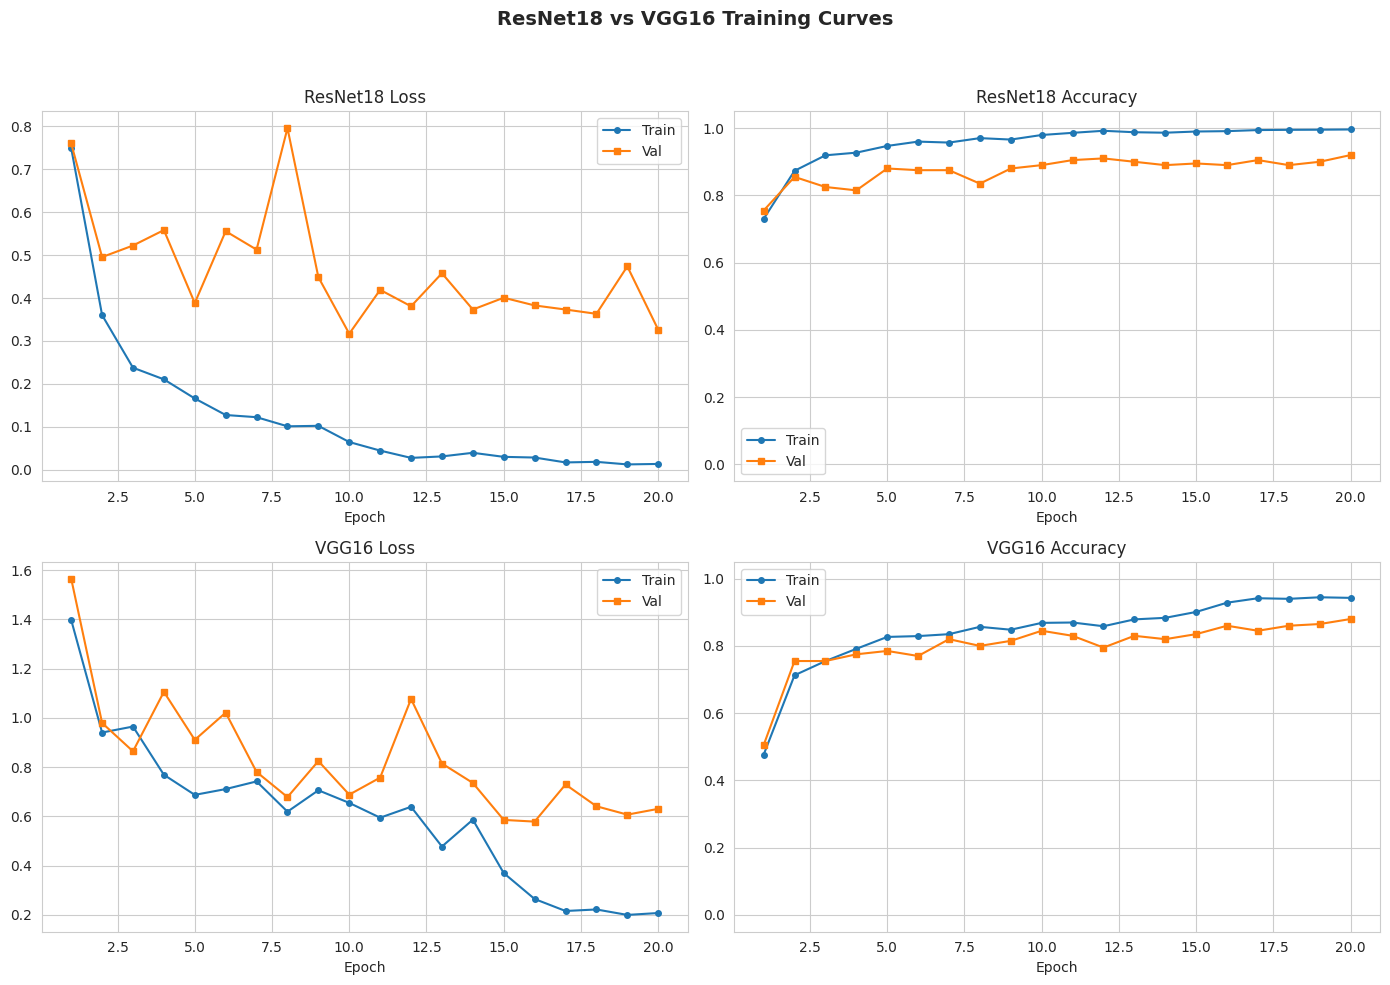
\includegraphics[width=0.88\linewidth]{../results/training_curves.png}
\caption{Training and validation loss/accuracy over 20 epochs.}
\label{fig:curves}
\end{figure}

\subsection{Test-Set Performance}

\begin{table}[H]
\centering
\caption{Test-set metrics (weighted average). Best in bold.}
\label{tab:metrics}
\begin{tabular}{@{}lcccc@{}}
\toprule
\textbf{Model} & \textbf{Accuracy} & \textbf{Precision} & \textbf{Recall} & \textbf{F1} \\
\midrule
ResNet18 & \textbf{0.900} & \textbf{0.904} & \textbf{0.900} & \textbf{0.900} \\
VGG16    & 0.873 & 0.879 & 0.873 & 0.874 \\
\bottomrule
\end{tabular}
\end{table}

\subsection{Confusion Matrices}

The most common misclassifications are between Neutral and Bored/Tired (both involve minimal facial movement) and between Confused and Neutral (subtle brow differences). ResNet18 has fewer errors overall.

\begin{figure}[H]
\centering
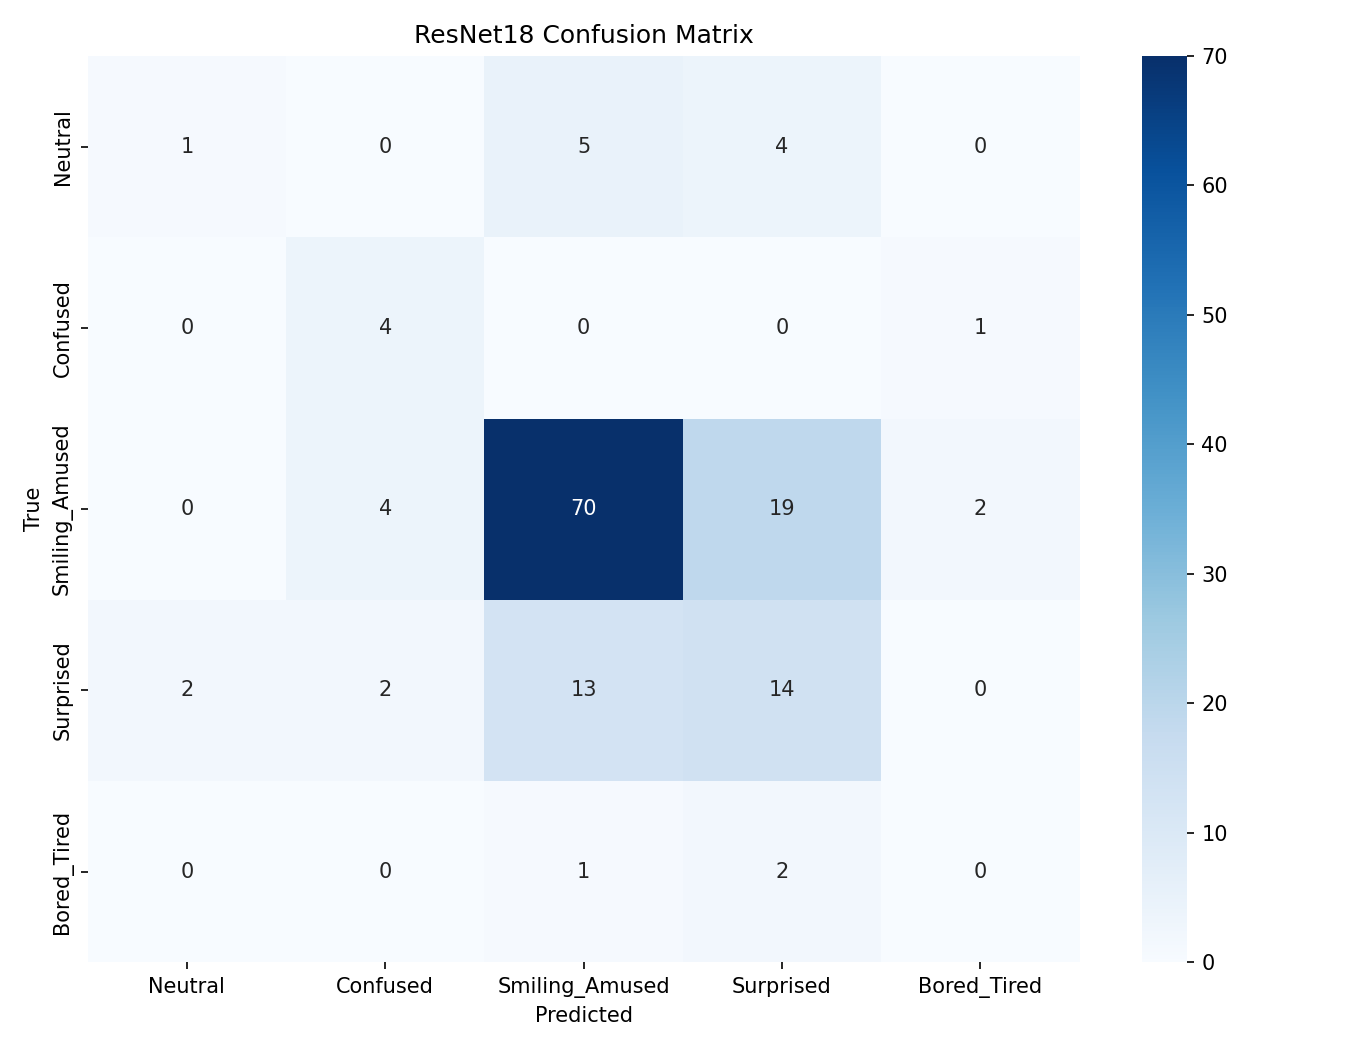
\includegraphics[width=0.49\linewidth]{../results/resnet18_confusion_matrix.png}\hfill
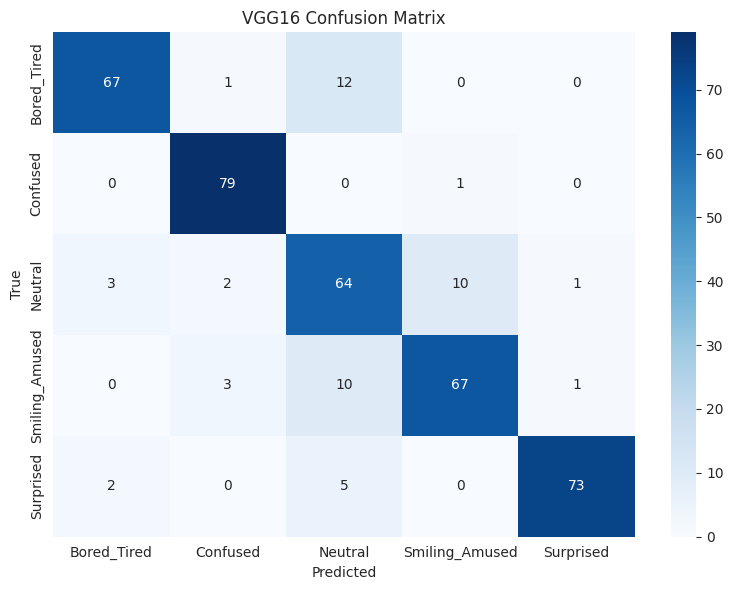
\includegraphics[width=0.49\linewidth]{../results/vgg16_confusion_matrix.png}
\caption{Confusion matrices: ResNet18 (left) and VGG16 (right).}
\label{fig:cm}
\end{figure}

\subsection{Grad-CAM Analysis}

Grad-CAM~\cite{selvaraju2017grad} heatmaps (Fig.~\ref{fig:gradcam}) show where the model looks when making predictions. For correct predictions, attention focuses on the face (brow, eyes). For misclassified crops, attention drifts to the background or shoulders, suggesting the model falls back on contextual shortcuts when the facial signal is weak.

\begin{figure}[H]
\centering
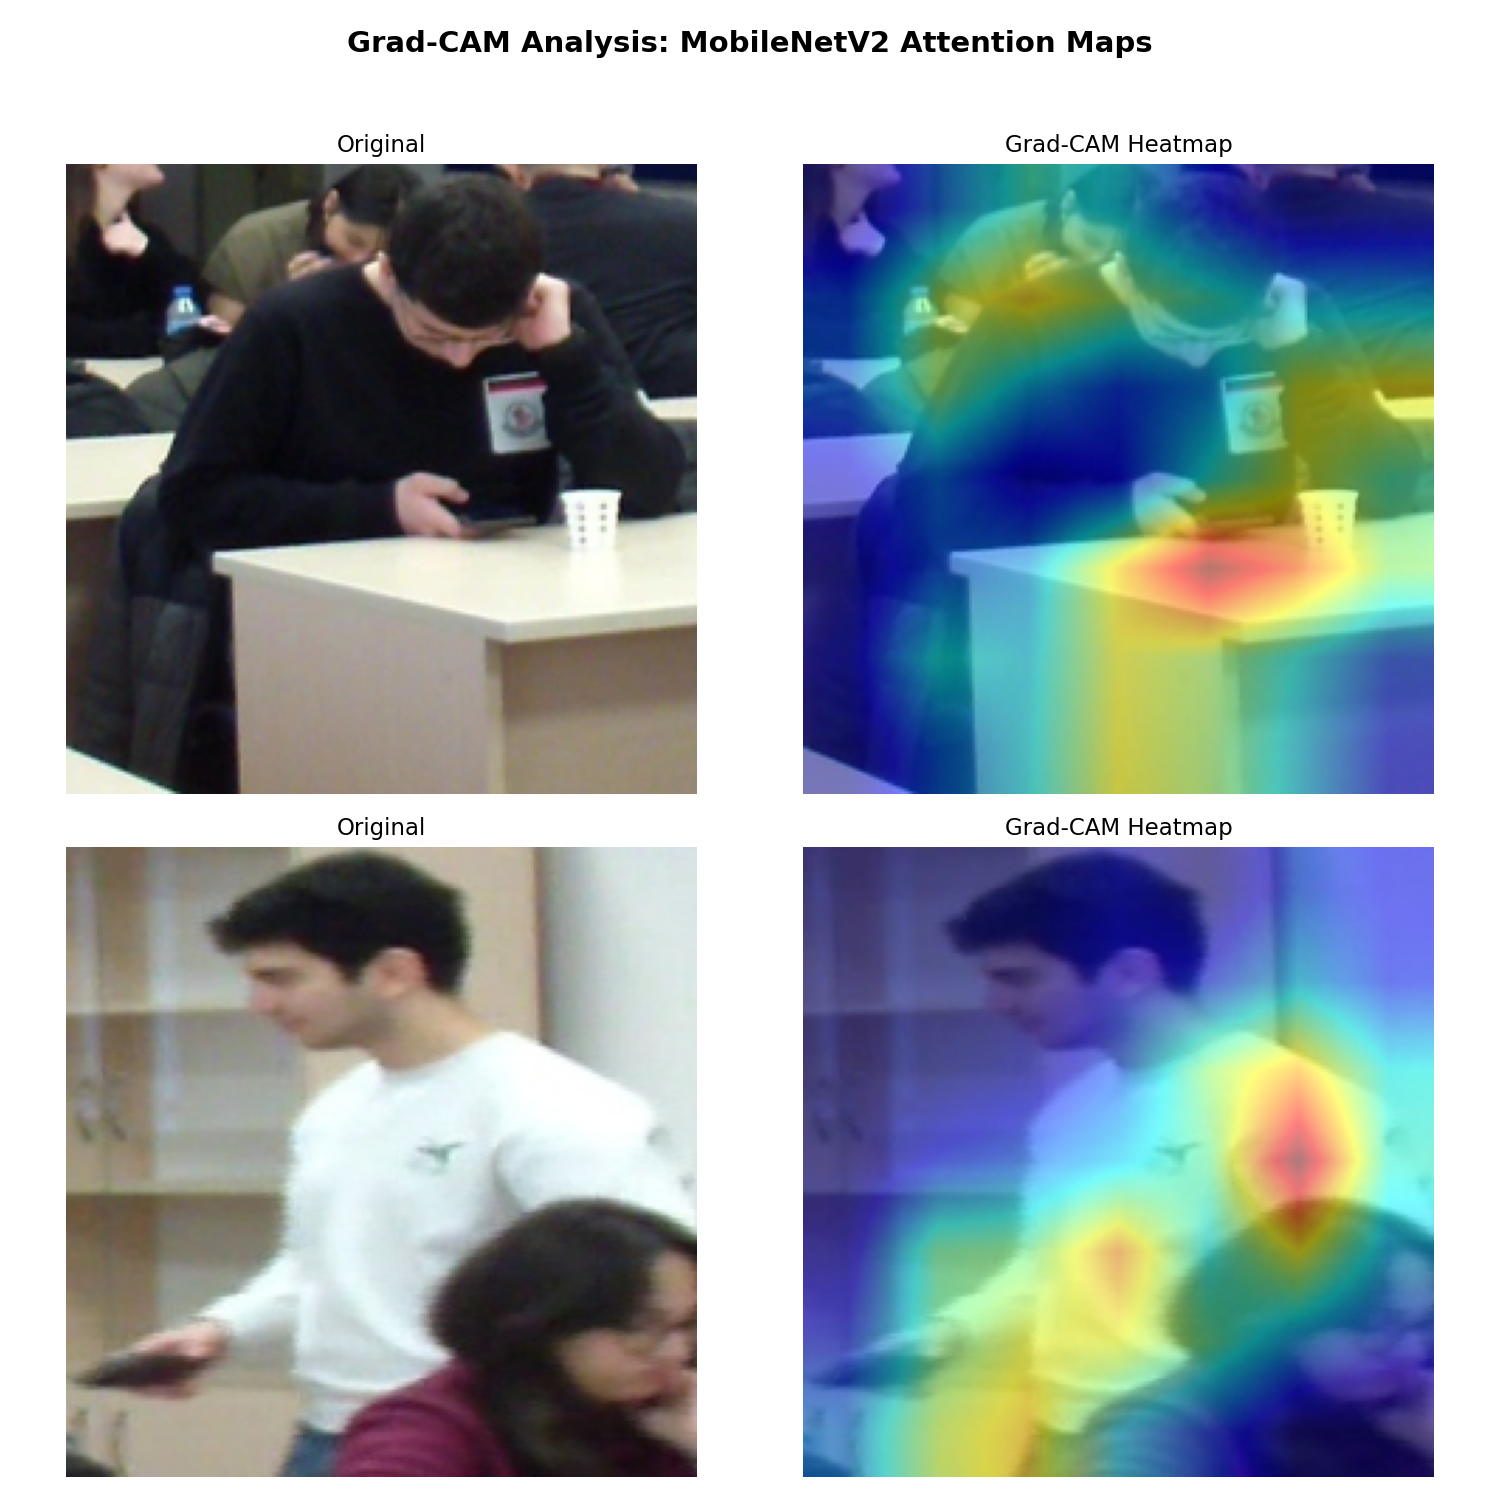
\includegraphics[width=0.75\linewidth]{../results/gradcam_analysis.png}
\caption{Grad-CAM heatmaps: correct prediction (left) vs.\ misclassification (right).}
\label{fig:gradcam}
\end{figure}

\subsection{t-SNE Feature Visualization}

Fig.~\ref{fig:tsne} projects ResNet18's internal features into 2D using t-SNE~\cite{vandermaaten2008tsne}. Smiling/Amused and Surprised form clear clusters. Neutral, Confused, and Bored/Tired overlap, confirming that these low-arousal expressions are genuinely hard to distinguish.

\begin{figure}[H]
\centering
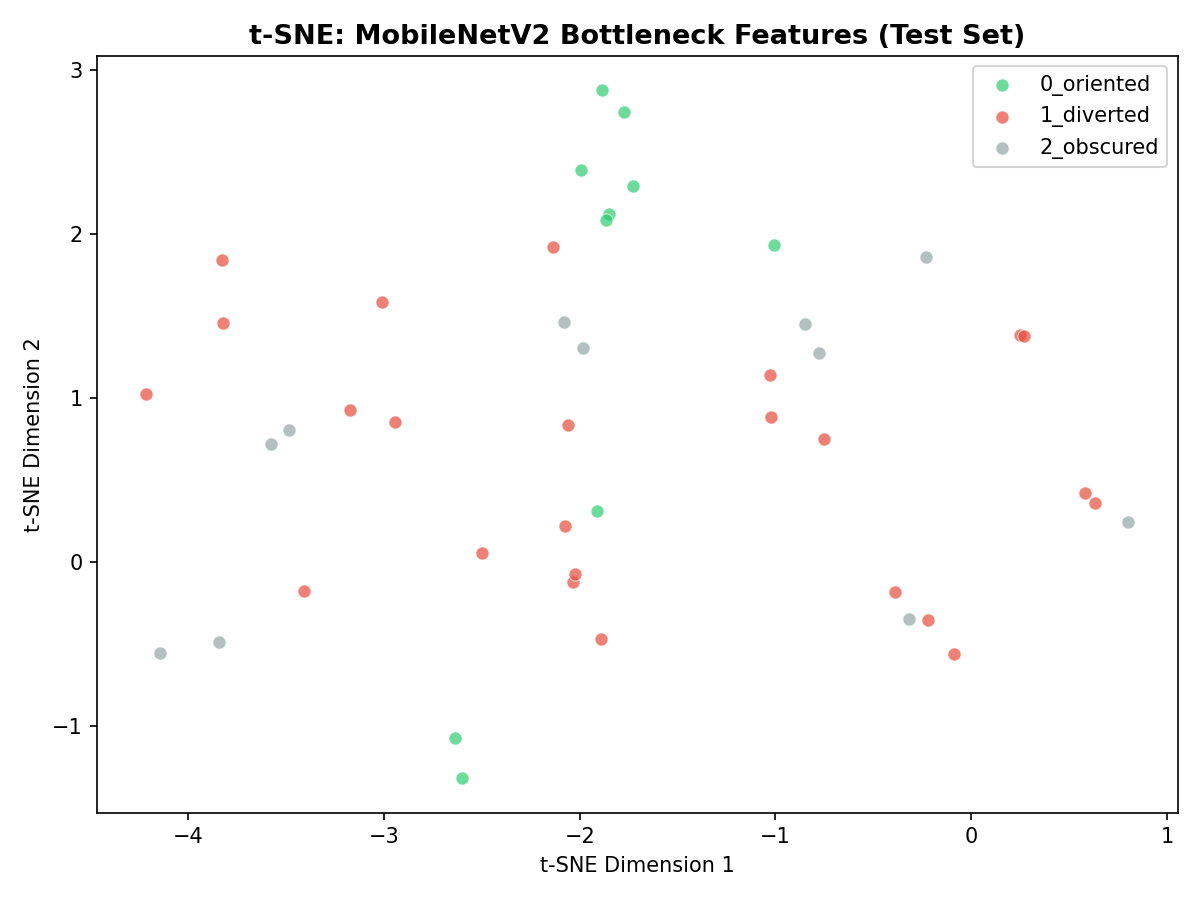
\includegraphics[width=0.68\linewidth]{../results/tsne_clusters.png}
\caption{t-SNE of ResNet18 test-set features.}
\label{fig:tsne}
\end{figure}

\subsection{ONNX Benchmark}

\begin{table}[H]
\centering
\caption{ResNet18: PyTorch vs.\ ONNX Runtime on CPU.}
\label{tab:onnx}
\begin{tabular}{@{}lccc@{}}
\toprule
\textbf{Runtime} & \textbf{Latency (ms)} & \textbf{FPS} & \textbf{Size (MB)} \\
\midrule
PyTorch    & 22.37  & 44.7  & 42.72 \\
ONNX (CPU) & \textbf{7.74} & \textbf{129.3} & 42.64 \\
\bottomrule
\end{tabular}
\end{table}

ONNX Runtime is $2.89\times$ faster than PyTorch on CPU. At 129 crops/second, this comfortably handles a classroom of 20--30 students at 1 FPS.

\subsection{Telemetry Dashboard}

The pipeline also generates a temporal view (Fig.~\ref{fig:telemetry}) showing how reaction proportions change across the lecture, smoothed with a rolling average. Sustained rises in Confused counts can flag difficult topic segments.

\begin{figure}[H]
\centering
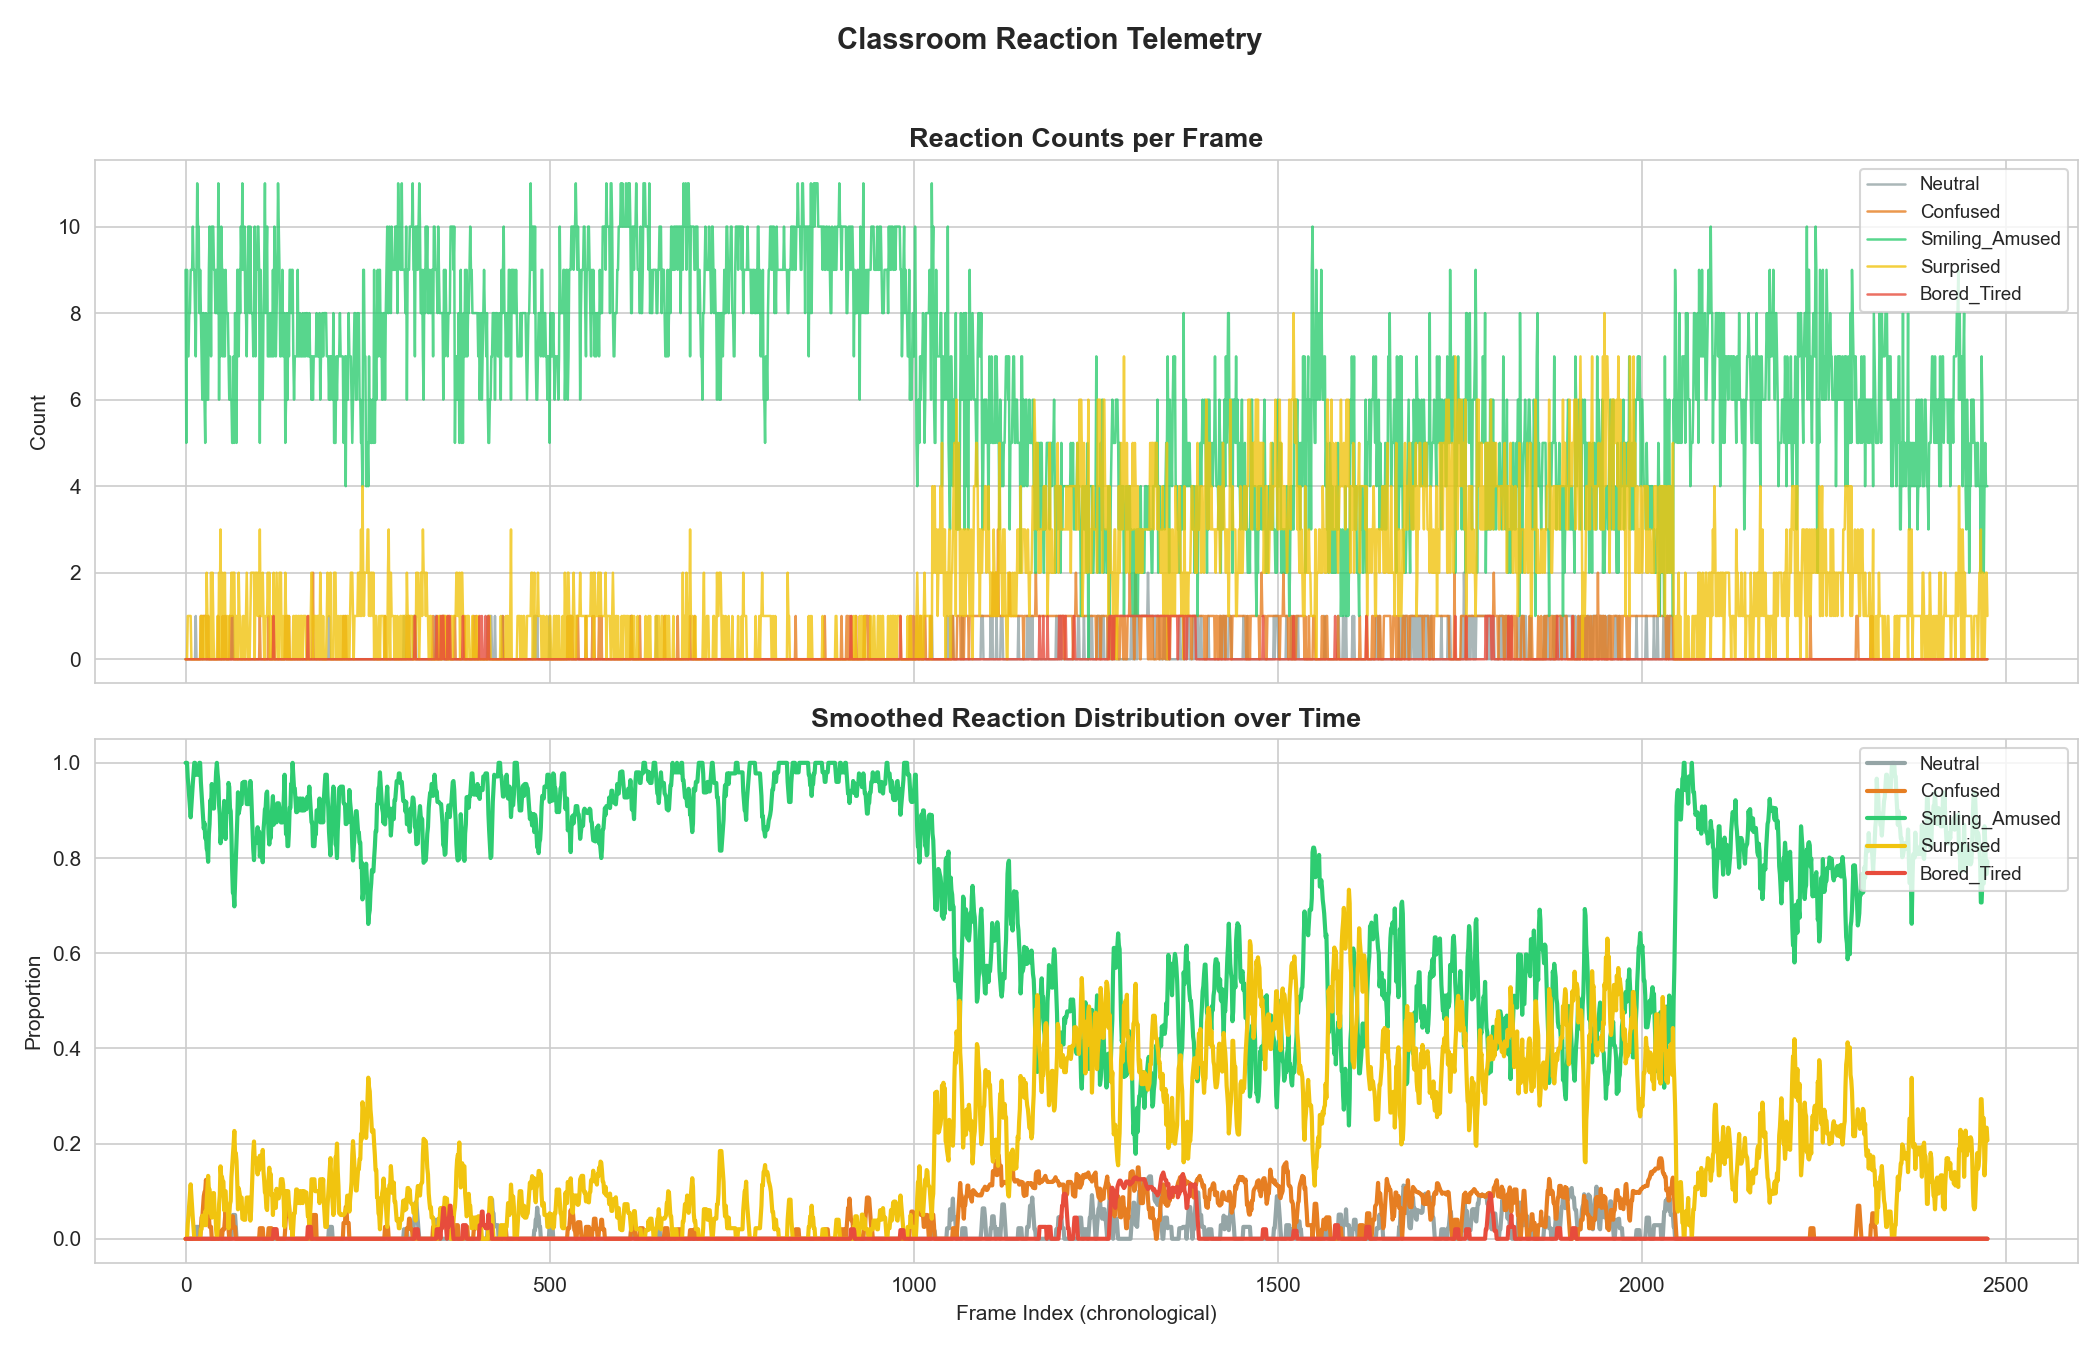
\includegraphics[width=0.88\linewidth]{../results/classroom_telemetry_dashboard.png}
\caption{Reaction telemetry across a lecture session.}
\label{fig:telemetry}
\end{figure}

% -----------------------------------------------------------------
\section{Cloud Architecture}

We designed a reference AWS architecture (Fig.~\ref{fig:aws}) for scaling the system to multiple classrooms:

\textbf{Edge:} AWS Greengrass runs the ONNX model on-device. Only JSON telemetry is sent upstream---raw video stays local for privacy.

\textbf{Real-time (hot path):} IoT Core $\to$ Kinesis Firehose $\to$ Amazon Timestream. Grafana dashboards show live reaction distributions. CloudWatch Alarms trigger Lambda for automated alerts.

\textbf{Historical (cold path):} Firehose also lands JSON logs in S3. Amazon Athena lets researchers run SQL queries over semesters of data without provisioning servers.

\textbf{MLOps:} SageMaker retrains models on accumulated S3 data and pushes updated ONNX weights back to edge devices via Greengrass OTA. AWS KMS encrypts all data at rest for FERPA/GDPR compliance.

\begin{figure}[H]
\centering
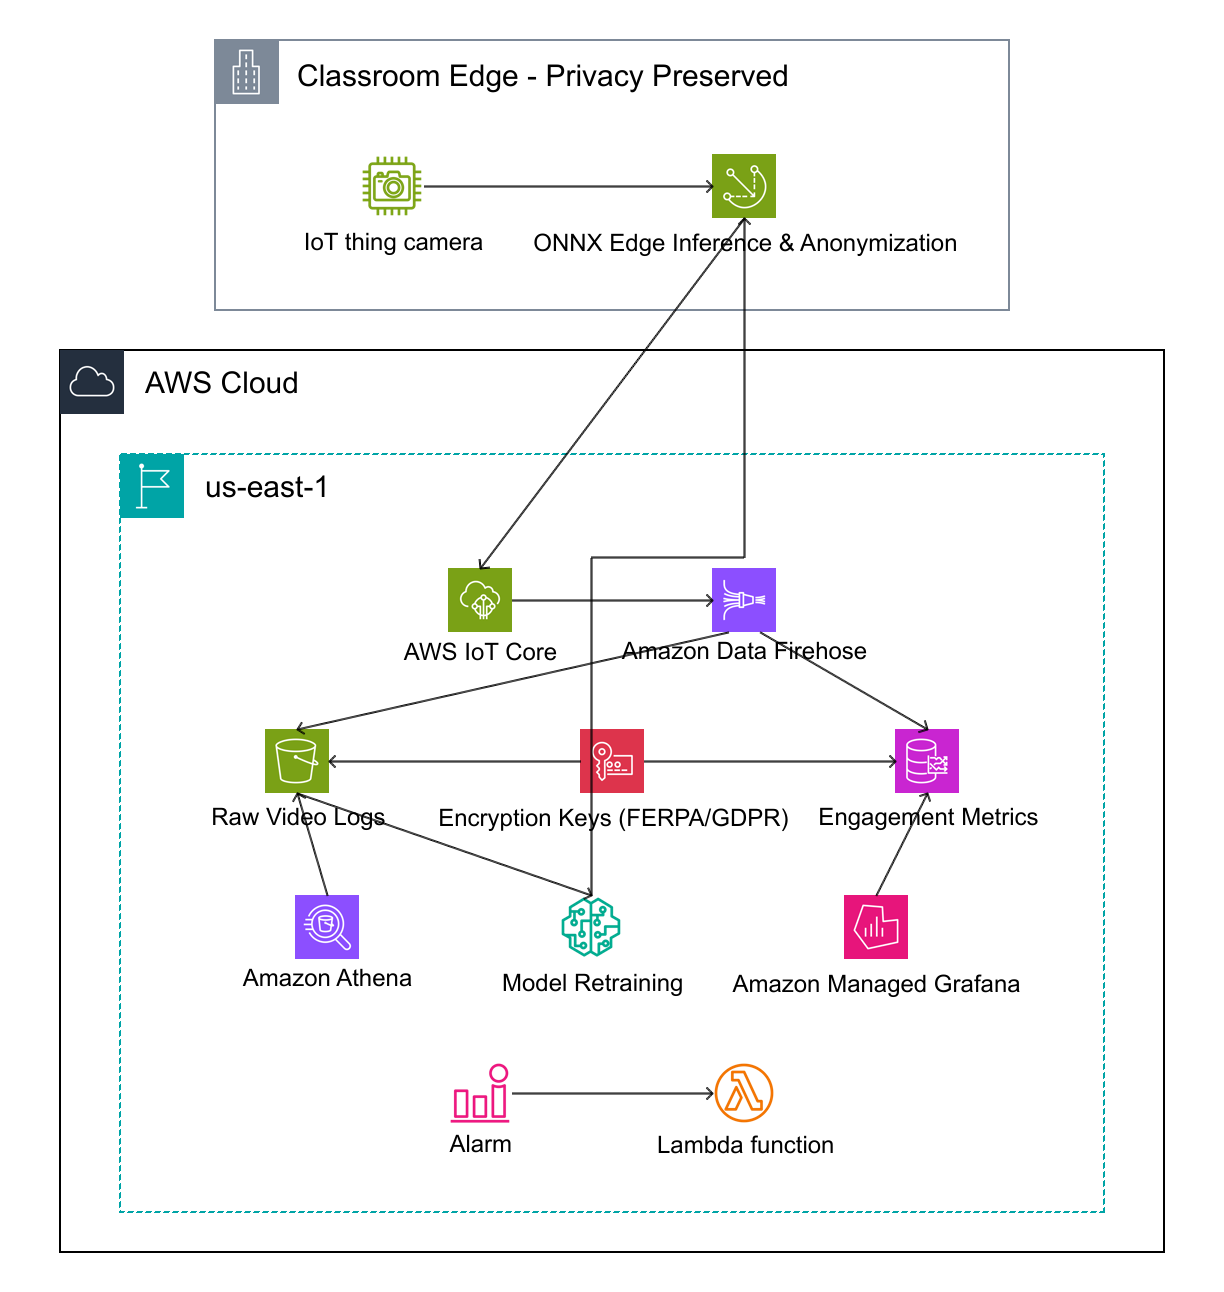
\includegraphics[width=\linewidth]{../results/aws_enterprise_architecture.png}
\caption{AWS architecture: edge inference, dual hot/cold analytics, and SageMaker retraining loop.}
\label{fig:aws}
\end{figure}

% -----------------------------------------------------------------
\section{Challenges and Lessons Learned}

\textbf{Small dataset from a single source.} With only 2\,000 crops from one classroom, the models risk learning scene-specific cues (backgrounds, seating) instead of generalizable facial features. The t-SNE overlap between low-arousal classes confirms this limitation.

\textbf{Annotation subjectivity.} The boundary between Neutral and Bored/Tired, or Neutral and Confused, is genuinely ambiguous. We discarded unclear crops, but did not compute formal inter-annotator agreement, so label noise likely affected both training and evaluation.

\textbf{Class imbalance.} Neutral and Smiling/Amused dominated the dataset. We addressed this with weighted loss and oversampling, which improved minority-class recall substantially, but Surprised and Confused still had lower recall than majority classes. No single technique fully solved the imbalance---combining weighted loss, oversampling, and augmentation together gave the best results.

\textbf{Fine-tuning depth matters.} ResNet18 (with \texttt{layer4} unfrozen) consistently outperformed VGG16 (classifier-only). This shows that for domain-specific tasks, adapting deeper feature layers is worth the overfitting risk when the dataset is small but augmented.

\textbf{Evaluation beyond accuracy.} Confusion matrices revealed the Neutral/Bored confusion that overall accuracy hid. Grad-CAM showed the model sometimes attends to background instead of faces. t-SNE showed which classes genuinely overlap in feature space. Each visualization tool revealed something that a single accuracy number could not.

% -----------------------------------------------------------------
\section{Conclusion}

We built a complete pipeline for classifying student reactions from classroom video. ResNet18 achieved 90.0\% accuracy, outperforming VGG16 (87.3\%) due to deeper fine-tuning. ONNX export made inference $2.89\times$ faster on CPU. The main limitations are the small, single-source dataset and the inherent ambiguity of subtle expressions. Future work could add temporal modeling (LSTM/Transformer over frame sequences), collect data from multiple classrooms, and use Vision Transformers for better accuracy on subtle expressions.

\section*{Acknowledgment}

This report was prepared for the course \emph{AI and ML Fundamentals} at Baku Higher Oil School (BHOS), instructed by Mirakram Aghalarov.

\begin{thebibliography}{00}

\bibitem{he2016deep}
K.~He, X.~Zhang, S.~Ren, and J.~Sun, ``Deep residual learning for image recognition,'' in \emph{Proc.\ IEEE CVPR}, 2016, pp.~770--778.

\bibitem{simonyan2015very}
K.~Simonyan and A.~Zisserman, ``Very deep convolutional networks for large-scale image recognition,'' in \emph{Proc.\ ICLR}, 2015.

\bibitem{jocher2023yolo}
G.~Jocher, A.~Chaurasia, and J.~Qiu, ``Ultralytics YOLOv8,'' 2023. [Online]. Available: \url{https://github.com/ultralytics/ultralytics}

\bibitem{selvaraju2017grad}
R.~R. Selvaraju et al., ``Grad-CAM: Visual explanations from deep networks via gradient-based localization,'' in \emph{Proc.\ IEEE ICCV}, 2017, pp.~618--626.

\bibitem{vandermaaten2008tsne}
L.~van~der~Maaten and G.~Hinton, ``Visualizing data using t-SNE,'' \emph{JMLR}, vol.~9, pp.~2579--2605, 2008.

\end{thebibliography}

\end{document}
